% IEEE standard conference template; to be used with:
%   spconf.sty  - LaTeX style file, and
%   IEEEbib.bst - IEEE bibliography style file.
% --------------------------------------------------------------------------

\documentclass[letterpaper]{article}
\usepackage{spconf,amsmath,amssymb,graphicx}
\usepackage{hyperref,url}

\usepackage{graphicx}
\usepackage[x11names, rgb]{xcolor}
\usepackage[figuresright]{rotating}
\usepackage{pgfplots}
\usepackage{tikz}
\pgfplotsset{compat=1.10}
\usepgfplotslibrary{fillbetween}
\usetikzlibrary{snakes,arrows,shapes,plotmarks,calc}

\newcommand\Top{\rule{0pt}{3ex}}
\newcommand\Bot{\rule[-1.5ex]{0pt}{0pt}}

% Monokai colors
\definecolor{color0}{HTML}{272822}
\definecolor{color1}{HTML}{383830}
\definecolor{color2}{HTML}{49483E}
\definecolor{color3}{HTML}{75715E}
\definecolor{color4}{HTML}{A59F85}
\definecolor{color5}{HTML}{F8F8F2}
\definecolor{color6}{HTML}{F5F4F1}
\definecolor{color7}{HTML}{F9F8F5}
\definecolor{color8}{HTML}{F92672}
\definecolor{color9}{HTML}{FD971F}
\definecolor{color10}{HTML}{F4BF75}
\definecolor{color11}{HTML}{A6E22E}
\definecolor{color12}{HTML}{A1EFE4}
\definecolor{color13}{HTML}{66D9EF}
\definecolor{color14}{HTML}{AE81FF}
\definecolor{color15}{HTML}{CC6633}
\newcommand\showcolors{

\begin{tikzpicture}
  \foreach \pos/\col in {0em/color0, 1em/color1, 2em/color2, 3em/color3, 
  4em/color4, 5em/color5, 6em/color6, 7em/color7, 8em/color8, 9em/color9, 
  10em/color10, 11em/color11, 12em/color12, 13em/color13, 14em/color14, 
  15em/color15}
  \fill[\col] (\pos,0) rectangle +(1em, 0.6em);
\end{tikzpicture}
}

% Example definitions.
% --------------------
% nice symbols for real and complex numbers
\newcommand{\R}[0]{\mathbb{R}}
\newcommand{\C}[0]{\mathbb{C}}

% bold paragraph titles
\newcommand{\mypar}[1]{{\bf #1.}}

% Title.
% ------
\title{Parallel build of randomized k-d trees and fast approximate kNN search on Xeon Phi}
%
% Single address.
% ---------------
% \name{Markus P\"uschel\thanks{The author thanks Jelena Kovacevic. This paper
% is a modified version of the template she used in her class.}} 
% \address{Department of Computer Science\\ ETH Z\"urich\\Z\"urich, Switzerland}

% For example:
% ------------
%\address{School\\
%		 Department\\
%		 Address}
%
% Two addresses (uncomment and modify for two-address case).
% ----------------------------------------------------------
\twoauthors%
{P. Santhanam\sthanks{psanthan@student.ethz.ch}, J. C. de Fine 
Licht\sthanks{definelj@student.ethz.ch}}%
{ETH Z\"urich\\%
Department of Computer Science\\%
Universit\"atstrasse 6, 8006 Z\"urich}%
{F. Wermelinger\sthanks{fabianw@mavt.ethz.ch}}%
{ETH Z\"urich\\%
% Computational Science and Engineering Laboratory\\%
Chair of Computational Science\\%
Clausiusstrasse 33, 8092 Z\"urich}%

\begin{document}
%\ninept
\maketitle

\begin{abstract}
    Nearest neighbour search across huge amount of data with high dimensionally finds its applications in image recognition (To Do: Other Applications). These applications demand the retrieval of k-nearest neighbours to be faster. KD Tree is an accelerating data structure which can perform the search faster on the low dimensional big data set. Performance of kd tree drops to that of the linear search when it is applied for high dimensional data. By inducing approximation over the retrieved search results randomised KD trees can perform the nearest neighbour look ups faster even over the high dimensional data. KD Trees and Randomised KD trees involve a build phase overhead. This might even be a bigger problem if the input data changes frequently and we need to build the Randomised KD forest in real time.( TO DO: Abstract of How do we parallelise and etc..)
\end{abstract}

% Mainbody
\section{Introduction}
  \label{sec:intro}

  % Do not start the introduction with the abstract or a slightly modified
  % version. It follows a possible structure of the introduction. 
  % Note that the structure can be modified, but the
  % content should be the same. Introduction and abstract should fill at most the first page, better less.

  \mypar{Motivation} In many applications, efficient search algorithms are of 
  great importance due to their high computational cost.  A common search 
  operation is to find a closest neighbor given some query point, which is 
  referred to as \emph{nearest neighbor search}.  This operation can readily be 
  extended to find the set of the $k$-nearest neighbors instead of just the 
  closest nearest neighbor.  The search space is usually very large and each 
  data point in such a set can be of high dimensionality.  For example, 
  matching images using distinct local image features~\cite{lowe2004a} is 
  a common task performed by web-search engines or in image recognition using 
  large datasets of up to $80$~million small images~\cite{torralba2008a}, where 
  each of the images is a high dimensional data point, depending on the number 
  of pixels used to represent the image.

  In order to speed-up the basic linear traversal of the data during the 
  search, accelerating data structures are employed.  For example, the k-d tree 
  is a simple space partitioning data structure~\cite{bentley1975a,friedman1977a}, where at each level a particular axis among the $k$ dimensions is chosen to split the points in the space.  However, exact 
  nearest neighbor search using a k-d tree is only efficient for low dimensional 
  data~\cite{muja2009a}.  For high dimensional data approximate structures, 
  such as a randomized k-d tree~\cite{silpa2008a} or hierarchical $k$-means 
  tree~\cite{muja2009a}, are used at the cost of the accuracy of the returned 
  nearest neighbors.

  In contrast to the naive linear search, an additional overhead is created by 
  building the accelerating data structure before performing the search.  
  Hence, the overall search time is composed of a build time for the data 
  structure and the time to perform the search using the structure.  Naturally, 
  the build time for a linear search vanishes.

  In this work, we focus on the fast parallel build of a set of randomized 
  k-d trees used to perform a parallel $k$-nearest neighbor search on high 
  dimensional data.  For our parallel application, we utilize the Intel many 
  integrated core (MIC) architecture offered by the Intel Knights Corner (KNC) 
  co-processor family.

  % \mypar{Motivation} The first task is to motivate what you do.  You can
  % start general and zoom in one the specific problem you consider.  In
  % the process you should have explained to the reader: what you are doing,
  % why you are doing, why it is important (order is usually reversed).

  % For example, if my result is the fastest sorting implementation ever, one
  % could roughly go as follows. First explain why sorting is important
  % (used everywhere with a few examples) and why performance matters (large datasets,
  % realtime). Then explain that fast implementations are very hard and
  % expensive to get (memory hierarchy, vector, parallel). 

  % Now you state what you do in this paper. In our example: 
  % presenting a sorting implementation that is
  % faster for some sizes as all the other ones.

  \mypar{Related work} Silpa-Anan and Hartley~\cite{silpa2008a} have proposed 
  a k-d tree algorithm based on creating multiple randomized k-d trees, where 
  each of the randomized trees splits the data based on a random choice of the 
  $D$ dimensions with highest variance.  Muja and Lowe have developed a C++ 
  library\footnote{\url{http://www.cs.ubc.ca/research/flann/}} for fast 
  approximate nearest neighbor searches with automatic algorithm selection 
  based on the data used for the search~\cite{muja2009a,muja2014a}.  The same 
  library implements a parallel build of a k-d tree for $3$D~data using GPU 
  hardware.  Building trees for high dimensional data is not parallelized.  The 
  work of Garcia~et~al.\@ employ GPUs to perform basic linear $k$-nearest 
  neighbor searches by using optimized linear algebra libraries and sorting 
  algorithms~\cite{garcia2008a,garcia2010a}.

  % \mypar{Related work} Next, you have to give a brief overview of
  % related work. For a report like this, anywhere between 2 and 8
  % references. Briefly explain what they do. In the end contrast to what
  % you do to make now precisely clear what your contribution is.

  % mainfile: ./../report.tex

\section{$k$-Nearest Neighbor Search}
  %\label{sec:_k_nearest_neighbor_search_algorithm}
  \label{sec:background}

  In this section we formally define the $k$-nearest neighbor search problem 
  and introduce the algorithm to build a randomized k-d tree.

  \mypar{Nearest neighbor search} Consider a set of points $\mathcal{P} 
  = \{p_1,p_2,\dots,p_n\}$ in a metric space $\mathbb{M}$ which defines some 
  distance function $d\colon\mathbb{M}\times\mathbb{M}\to\mathbb{R}$.  If we 
  are given a query point $q\in\mathcal{P}$, the nearest neighbor of $q$ must 
  satisfy the condition
  \begin{align}
    \label{eq:NN}
    \operatorname{NN}(q,\mathcal{P}) &= \operatorname{argmin}_{x\in\mathcal{P}} 
    d(q,x)\in\mathcal{P}.
  \end{align}

  Often we are not interested in only one nearest neighbor, but the $k$~nearest 
  neighbors, for which we use the notation
  \begin{align}
    \label{eq:kNN}
    \operatorname{kNN}(q,\mathcal{P},k) &= \mathcal{A},
  \end{align}
  where $\mathcal{A}\subseteq\mathcal{P}$ with cardinality 
  $\vert\mathcal{A}\vert = k$.  The following constraint must further be 
  satisfied
  \begin{align}
    \label{eq:constraint_kNN}
    \{d(q,x)\mid d(q,x)\leq d(q,y)\forall x\in\mathcal{A}, 
    y\in\mathcal{P}-\mathcal{A},q\in\mathcal{P}\}.
  \end{align}
  Since the cardinality of $\mathcal{A}$ is $k$, it follows that $n\geq k$ for 
  the number of points in $\mathcal{P}$.

  \mypar{Randomized k-d~tree build} Building the tree is similar to a conventional 
  k-d tree as described in~\cite{bentley1975a,friedman1977a}, but rather than choosing the dimension used to split the data deterministically, 
  the data is split % in a $d$-dimensional metric space along 
  in along some dimension $d$ chosen randomly among the $D$ dimensions with highest variance. Each point 
  $\pmb{p}\in\mathcal{P}$, for which the value of the $p_i$ dimension is lower than 
  the value of the median in the chosen dimension at the current node, is 
  placed in a reduced set of points $\mathcal{P}_l\subset\mathcal{P}$ or 
  $\mathcal{P}_r\subset\mathcal{P}$ otherwise, where 
  $\mathcal{P}_l\cup\mathcal{P}_r = \mathcal{P}$.
  The procedure is then recursively applied to the two new branches using the 
  corresponding set of points $\mathcal{P}=\mathcal{P}_l$ or 
  $\mathcal{P}=\mathcal{P}_r$ with a new random choice for the split dimension 
  $d$. % The recursion bottoms out for $\left|P\right|=1$, where the remaining point is stored as a leaf, resulting in a total of $2\left|P\right|-1$ nodes.
  % For the work presented here, we follow~\cite{muja2009a} and set $D=5$.
  
  \mypar{Randomized k-d~tree search}
Multiple randomized k-d trees are searched for $k$ nearest neighbors. For each query two bounded heaps $H_{1}$ and $H_{2}$ are maintained across the randomized k-d forest. $H_{1}$ tracks the $k$ closest neighbors and $H_{2}$ maintains the most promising branches not yet searched across all trees according to the distance from the query point their along their split dimension. The algorithm first recurses to the bottom once, storing the most promising branches encounted during
the recursion in $H_{2}$, then pops the lowest distance branch from $H_{2}$ and repeats the process. After inspecting some maximum number of leaves $m<\left|\mathcal{P}\right|$ among all the randomized trees, the search returns the $k$ closest neighbors found as an approximation of the true $k$ nearest neighbors. As such, $m$ is the parameter that determines the trade-off between accuracy and speed ($m=\left|\mathcal{P}\right|$ falls back to the conventional k-d tree
algorithm, returning an exact result).
  % Give a short, self-contained summary of necessary
  % background information. For example, assume you present an
  % implementation of sorting algorithms. You could organize into sorting
  % definition, algorithms considered, and asymptotic runtime statements. The goal of the
  % background section is to make the paper self-contained for an audience
  % as large as possible. As in every section
  % you start with a very brief overview of the section. Here it could be as follows: In this section 
  % we formally define the sorting problem we consider and introduce the algorithms we use
  % including a cost analysis.

  % \mypar{Sorting}
  % Precisely define sorting problem you consider.

  % \mypar{Sorting algorithms}
  % Explain the algorithm you use including their costs.

  % As an aside, don't talk about "the complexity of the algorithm.'' It's incorrect,
  % problems have a complexity, not algorithms.

  % mainfile: ./../report.tex

\section{Parallelization Schemes}
  % \label{sec:parallelisation_schemes}
  \label{sec:method}

This section describes the approaches to parallelize build and search process
 of the randomized k-d trees. 

\mypar{Build Parallization}
If $N$ is the number of randomized k-d trees to be built, the trivial first
 layer of parallelism is building these $N$ trees in parallel.

Intel's Threading Building Blocks (TBB) %\footnote{\url{https://www.threadingbuildingblocks.org/}}
is a widely used C++ template library for
task parallelism. TBB's uses work stealing to schedule tasks, abstracted in the high level construct \texttt{tbb::task\_group}. Each randomized k-d tree is built by recursively splitting the input points as described in Section~\ref{sec:background}.
Whenever a split occurs, the workload is partitioned into a recursion on $\mathcal{P}_l$ and on $\mathcal{P}_r$, corresponding to two equally sized tasks. These can then be submitted to the TBB scheduler to be treated by distinct threads. Since the work is completely balanced at each split due to splitting on the median, recursion level $i$ will be running a total of $2i$ tasks. To avoid additional overhead, spawning of new tasks is stopped when all available threads are occupied. Because
$N$ trees are built in parallel, a given task will perform the rest of the recursion when $2 i N\geq P$ without spawning new tasks, where $P$ is the amount of processors available.
%  at each
%     node the set of points $\mathcal{P}$ into $\mathcal{P}_{l}$ and $\mathcal{P}_{r}$. Let $C$ denote the number of available hardware 
%     threads. $T_i$ denote the task of splitting the set of points $\mathcal{P}_{i}$ at the level $i$ into $\mathcal{P}_{l,i}$ and $\mathcal{P}_{r,i}$. The
%      Task group $G$ is obtained as
% \begin{align}
% G=\lbrace T_i \mid i \in [0,i_{max}] \rbrace
% \end{align} 
% \label{eq:tbb_task_group} 
% where $i_{max}$ is the level at which the width of the tree equals $C/N$.
%  The equation $\ref{eq:tbb_task_group}$  constrains the spanning of tasks
%   int the task group from the root till the width of the tree equals the number of available hardware threads. 

  \mypar{Search parallelization} Searching the randomized k-d trees can be parallelized trivially over input queries, as only read access to the trees is required. Each query $q_i$ maintains separate heaps $H_{i,1}$ and $H_{i,2}$ as described in Section~\ref{sec:background}. This is implemented using TBB's \texttt{parallel\_for} loop construct. 

  \mypar{Xeon Phi} The MIC architecture offered on the Xeon Phi is expected to be a good match to the randomized k-d tree search 
  due to several factors: firstly the highly parallel nature of the search 
  offers full hardware utilization when queried with a sufficiently high 
  numbers of points, while not being fully vectorizable due to the 
  heterogeneousness of the tree structure.
  Secondly, the algorithm offers benefits of sharing memory between caches 
  without causing performance hits due to writes. Thirdly, computing the 
  Euclidian distance between high dimensional input offers an opportunity to 
  take advantage of the 512-bit wide SIMD units on the Knight's Corner cores, 
  treating up to 16 single precision floating point numbers in parallel.  


 % Now comes the ``beef'' of the report, where you explain what you
%   did. Again, organize it in paragraphs with titles. As in every section
 %  you start with a very brief overview of the section.

 %  In this section, structure is very important so one can follow the technical content.

%   Mention and cite any external resources that you used including libraries or other code.

  % mainfile: ./../report.tex

\section{Experimental results}\sloppy
  \label{sec:exp}

  % Here you evaluate your work using experiments. You start again with a
  % very short summary of the section. The typical structure follows.
  %
  % \mypar{Experimental setup} Specify the platform (processor, frequency, maybe OS, maybe cache sizes)
  % as well as the compiler, version, and flags used. If your work is about performance, 
  % I strongly recommend that you play with optimization flags and consider also icc for additional potential speedup.
  %
  % Then explain what kind of benchmarks you ran. The idea is to give enough information so the experiments are reproducible by somebody else on his or her code.
  % For sorting you would talk about the input sizes. For a tool that performs NUMA optimization, you would specify the programs you ran.

  \mypar{Setup}
  Benchmarks were run on two distinct setups: a node of ETH's Euler cluster, 
  a convential x86 multicore platform, and on ETH's Einstein machine with 
  ssh-access to a Knight's Corner Intel Xeon Phi coprocessor. An Euler node 
  consists of two Intel Xeon E5-2697v2 processors for a total of 24 x86 cores 
  in a dual-socket NUMA setup. The x86 benchmark code was compiled with GCC 
  4.9.2 with OpenMP 4.0, while the Xeon Phi host code was compiled with GCC 
  4.8.2. Both setups used the precompiled version of TBB 4.4 provided by Intel for parallelization.
  \begin{figure}[tb]
    \centering
    \resizebox{\columnwidth}{!}{% File:   buildCompare.tex
% Date:   Mon Jan 18 20:54:14 2016
% Author: Fabian Wermelinger
% Tag:    Buidl comparison
% Copyright 2016 ETH Zurich. All Rights Reserved.
\begin{tikzpicture}[scale=0.7]
  \begin{semilogyaxis}[
    log basis y=10,
    grid=both,
    log ticks with fixed point,
    ymin=0.1,ymax=100,
    xtick={1, 2, 4, 6, 8, 12, 16, 18, 24},
    legend style={legend pos=north east, cells={anchor=west}, 
    font=\footnotesize},
    xlabel={Number of Cores},
    ylabel={Mean Build Time $[s]$}]

    % flann
    \addplot[mark=x, color0, error bars/.cd, y dir=both, y explicit, error bar 
    style={color3}] table[x index=0, y index=1, y error index=2] 
    {./03_results/figs/data_1M/flannBuild.dat};
    \addlegendentry{FLANN}

    % ours
    \addplot[mark=o, color8, error bars/.cd, y dir=both, y explicit, error bar 
    style={color0}] table[x index=0, y index=1, y error index=2] 
    {./03_results/figs/data_1M/randomizedBuild.dat};
    \addlegendentry{Our Implementation}

  \end{semilogyaxis}
\end{tikzpicture}
}
    \caption{Mean build time for the FLANN library and our implementation using 
    $1$~million SIFT vectors.}
    \label{fig:build_comparison}
  \end{figure}
  The Xeon Phi setup additionally uses the MPI library from Intel Parallel 
  Studio XE 2016 when communicating with the Xeon Phi on both host and 
  coprocessor, and the MIC code (\texttt{-mmic}) is compiled using ICC 15.0.0.  
  \begin{figure}[tb]
    \centering
    \resizebox{\columnwidth}{!}{% File:   buildSpeedup.tex
% Date:   Mon Jan 18 22:22:51 2016
% Author: Fabian Wermelinger
% Tag:    Buidl Speedup
% Copyright 2016 ETH Zurich. All Rights Reserved.
\begin{tikzpicture}[scale=0.7]
  \begin{axis}[
    grid=major,
    xtick={1, 2, 4, 6, 8, 12, 16, 18, 24},
    legend style={legend pos=south west, cells={anchor=west}, 
    font=\footnotesize},
    xlabel={Number of Cores},
    ylabel={Speedup Factor}]

    % speedup
    \addplot[mark=x, color8, error bars/.cd, y dir=both, y explicit, error bar 
    style={color0}] table[x index=0, y index=1, y error index=2] 
    {./03_results/figs/data_1M/buildSpeedup.dat};
  \end{axis}
\end{tikzpicture}
}
    \caption{Speedup over the FLANN library for building $4$ randomized k-d 
    trees.}
    \label{fig:build_speedup}
  \end{figure}
  All code was compiled with \texttt{-std=c++11} standard, \texttt{-O3} 
  optimization and \texttt{-march=native} SIMD vectorization (the Euler cluster supports 256-bit vector instructions) for both GCC and 
  ICC. % In particular computing Euclidian distances between high-dimensional input offers a potential gain of vectorization. 

  \mypar{Data set}
  Measurements are done on the TEXMEX~\cite{jegou2011} data set, which is 
  a collection of SIFT~\cite{lowe1999a,lowe2004a} descriptors: 128-dimensional 
  vectors of single precision floating points numbers invariantly describing features in images, commonly used in computer 
  vision to recognize transformations between images taken of the same 
  underlying content. The data set is produced specifically by the authors 
  of~\cite{jegou2011} to test the performance of nearest neighbor algorithms, 
  as it offers a high input size of
  high-dimensional data applied to a common real world problem.
  Comparisons between the vectors are done using the Euclidian distance between them for a relatively low computation intensity of $\approx3/4$ floating point operations per byte. Results presented below are run for the data set containing 1~million reference points queried with 10000 test points for $k=100$.  

  % \mypar{Results}
  % Next divide the experiments into classes, one paragraph for each. In each class of experiments you typically pursue one questions that then is answered by a suitable plot or plots. For example, first you may want to investigate the performance behavior with changing input size, then how your code compares to external benchmarks.
  %
  % For some tips on benchmarking including how to create a decent viewgraph see pages 22--27 in \cite{Pueschel:10}.
  %
  % {\bf Comments:}
  % \begin{itemize}
  %   \item Create very readable, attractive plots (do 1 column, not 2 column plots
  %     for this report) with readable font size. However, the font size should also not be too large; typically it is smaller than the text font size.
  %     An example is in Fig.~\ref{fftperf} (of course you can have a different style).
  %   \item Every plot answers a question. You state this question and extract the
  %     answer from the plot in its discussion.
  %   \item Every plot should be referenced and discussed.
  % \end{itemize}
  %
  % \begin{figure}\centering
  %   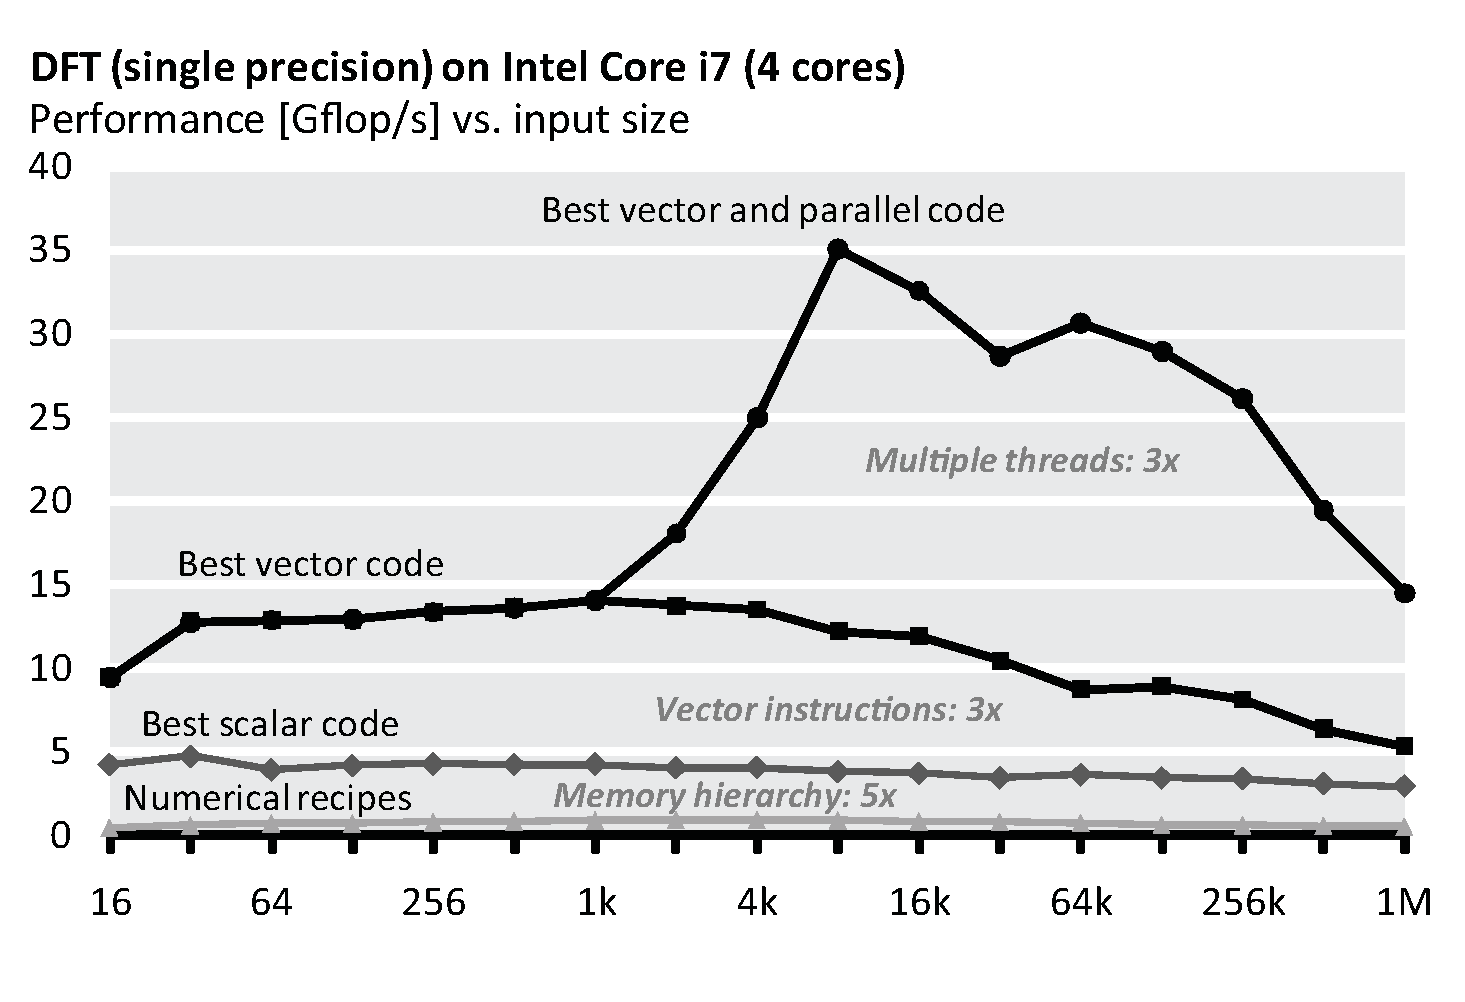
\includegraphics[scale=0.33]{./03_results/figs/dft-performance.eps}
  %   \caption{Performance of four single precision implementations of the
  %   discrete Fourier transform. The operations count is roughly the
  %   same. The labels in this plot are maybe a little bit too small.\label{fftperf}}
  % \end{figure}

  \mypar{Build performance} To evaluate the performance of the build 
  parallelization scheme described in Section~\ref{sec:method}, our 
  implementation is compared to the implementation provided by the FLANN 
  library. Because FLANN implements no parallelization of the tree build, 
  and in particular no trivial parallelization of building $N$ randomized trees in 
  parallel, the implementation described here must scale beyond $N$ processors 
  to demonstrate the advantage of the recursive task
  spawning scheme. In the below we fix $N=4$, as this is enough for satisfactory search performance, while only offering a small initial amount of trivial parallellism up to 4 cores.
  This work contains no demonstration of the suggested 
  parallel build scheme run on Xeon Phi, as compiling the code with ICC for 
  unknown reasons resulted in a build time two orders of magnitude higher than 
  when compiled with GCC, even when run exclusively on the host platform.
  \begin{figure}[tb]
    \centering
    \resizebox{\columnwidth}{!}{% File:   buildCompare.tex
% Date:   Mon Jan 18 20:54:14 2016
% Author: Fabian Wermelinger
% Tag:    Buidl comparison
% Copyright 2016 ETH Zurich. All Rights Reserved.
\begin{tikzpicture}[scale=0.7]
  \begin{semilogyaxis}[
    log basis y=10,
    grid=both,
    log ticks with fixed point,
    xtick={1, 2, 4, 6, 8, 12, 16, 18, 24},
    legend style={legend pos=north east, cells={anchor=west}, 
    font=\footnotesize},
    xlabel={Number of Cores},
    ylabel={Mean Search Time $[s]$}]

    % flann
    \addplot[mark=x, color0, error bars/.cd, y dir=both, y explicit, error bar 
    style={color3}] table[x index=0, y index=1, y error index=2] 
    {./03_results/figs/data_1M/flannSearch.dat};
    \addlegendentry{FLANN}

    % ours
    \addplot[mark=o, color8, error bars/.cd, y dir=both, y explicit, error bar 
    style={color0}] table[x index=0, y index=1, y error index=2] 
    {./03_results/figs/data_1M/randomizedSearch.dat};
    \addlegendentry{Our Implementation}

  \end{semilogyaxis}
\end{tikzpicture}
}
    \caption{Comparison against FLANN for a search of $10000$ query vectors 
    using $4$ randomized k-d trees.}
    \label{fig:search_comparison}
  \end{figure}
  The mean build time of the two implementations are compared 
  in Figure~\ref{fig:build_comparison}, while Figure~\ref{fig:build_speedup} shows the computed speedup over the FLANN 
  library. Because of the lack of parallelization in FLANN, Figure~\ref{fig:build_speedup} can be considered a strong scaling plot with the FLANN single core performance as the baseline. % All measurements shown here are obtained from the Euler compute cluster using one node with $24$ cores.
  The performance is seen to scale well beyond the initial parallel construction of 4 trees, and the build time is down to $0.55$ seconds when utilizing all 24 cores on an Euler node, a speedup of $11$ when compared to the FLANN baseline. This shows a significant benefit of the parallel tree build scheme. As seen for the first data point in Figure~\ref{fig:build_comparison}, the single core performance of FLANN is $45\%$ better than for our implementation, meaning that scalar
  optimizations to our code should have a significant positive impact on the speedup. 

  \mypar{Search performance} Since no novel work is done to improve over the 
  search algorithm implemented for randomized k-d trees in the FLANN library, 
  the performance of the implementation presented here is only expected to 
  match that of FLANN. The contribution of this work is to evaluate the 
  performance of the search algorithm on the Xeon Phi platform.   \begin{figure}[tb]
    \centering
    \resizebox{\columnwidth}{!}{% File:   buildSpeedup.tex
% Date:   Mon Jan 18 22:22:51 2016
% Author: Fabian Wermelinger
% Tag:    Buidl Speedup
% Copyright 2016 ETH Zurich. All Rights Reserved.
\begin{tikzpicture}[scale=0.7]
  \begin{axis}[
    grid=major,
    xtick={1, 2, 4, 6, 8, 12, 16, 18, 24},
    legend style={legend pos=south west, cells={anchor=west}, 
    font=\footnotesize},
    xlabel={Number of Cores},
    ylabel={Speedup Factor}]

    % speedup
    \addplot[mark=x, color8, error bars/.cd, y dir=both, y explicit, error bar 
    style={color0}] table[x index=0, y index=1, y error index=2] 
    {./03_results/figs/data_1M/searchSpeedup.dat};
  \end{axis}
\end{tikzpicture}
}
    \caption{Speedup of $100$-nearest neighbor search against the FLANN library for $10000$ 
    query vectors.}
    \label{fig:search_speedup}
  \end{figure}
  Because of the issues with the build algorithm compiled with ICC as described 
  above, search on the Xeon Phi is done by building the randomized trees on the 
  host processor, then transferring the tree structure using explicit MPI send and receive 
  calls. This allows the host and coprocessor binaries to be built and linked 
  separately with different compilers, relying on Intel's MPI library for 
  interfacing.
  Figure~\ref{fig:search_comparison} shows mean search time observed for a search of $10000$ query vectors using $4$ randomized k-d trees on both the Euler and Xeon Phi platforms, while Figure~\ref{fig:search_speedup} plots the speedup over the FLANN library. % The measurements have been conducted on one node of the Euler platform specified above.  The speedup based on these measurements relative to the FLANN library is shown in Figure~\ref{fig:search_speedup}.
  The scaling between our implementation and that of FLANN is seen in Figure~\ref{fig:search_speedup} to be very similar, but the performance on the Euler node is consistently a factor $0.4$-$0.6$ slower. As with the results for the parallel build described above, this means that our single core performance is lacking when compared to the FLANN library. Because the search parallelizes trivially, the data points in Figure~\ref{fig:search_speedup} are approximately measurements of the same
  number, namely the speedup of the single core performance, resulting in a large propagated error relative to the scale of the plot. The error on the measurements for 12 and 24 cores are considerably lower than the other data points, suggesting that the large deviation is due to jobs contesting resources when running on the Euler batch system and reserving less than the number of cores available on one or two full NUMA nodes.
  For the Xeon Phi the search is run on 240 threads, utilizing the 4 hyperthreads on each of the 60 available cores. The time to solution intersects that of the Euler node at around 12 cores, corresponding to a relative factor of $0.2$ performance per Xeon Phi core to Xeon core. The Xeon Phi numbers do not include the time spent on data transfer, but these numbers become negligible if utilizing the full PCI Express bus for the application described here. When tested for the purpose of this
  work, send/receive calls of MPI only offered $10\%$ of the memory bandwidth promised by PCI Express, while offload mode almost reached the data sheet performance. Even with this performance hit, memory transfers would only add $20\%$ to the total time to solution, down to $2\%$ if the full bandwidth was to be exploited. 

  % mainfile: ./../report.tex

\section{Conclusion}
\label{sec:conclusion}

% Here you need to summarize what you did and why this is
% important. {\em Do not take the abstract} and put it in the past
% tense. Remember, now the reader has (hopefully) read the report, so it
% is a very different situation from the abstract. Try to highlight
% important results and say the things you really want to get across
% such as high-level statements (e.g., we believe that .... is the right
% approach to .... Even though we only considered x, the
% .... technique should be applicable ....) You can also formulate next
% steps if you want. Be brief. After the conclusions there are only the references.

The parallel build scheme for randomized k-d trees presented here has been shown to scale to a high number of cores, reducing the build time for four trees from one million SIFT descriptors to roughly half a second on a node consisting of 24 cores. This makes it feasible to construct and query randomized k-d trees in real-time applications even for very large data sets. Search performance on the Xeon Phi was shown to match that of a single 12-core Xeon E5-2697v2 socket
without explicit Xeon Phi optimizations. Although this corresponds to a somewhat worse performance per dollar for this application (based on suggested retail price by Intel per January 2016), it incites some optimism to the potential of the coprocessor, especially for the introduction of the Knight's Landing generation, which should significantly improve cache performance, as well as doubling the number of available cores. 

% mainfile: ./../report.tex

% \section{Further Comments}
  \label{sec:further_comments}

  Here we provide some further tips.

  \mypar{Further general guidelines}

  \begin{itemize}
    \item For short papers, to save space, I use paragraph titles instead of
      subsections, as shown in the introduction.

    \item It is generally a good idea to break sections into such smaller
      units for readability and since it helps you to (visually) structure the story.

    \item The above section titles should be adapted to more precisely
      reflect what you do.

    \item Each section should be started with a very
      short summary of what the reader can expect in this section. Nothing
      more awkward as when the story starts and one does not know what the
      direction is or the goal.

    \item Make sure you define every acronym you use, no matter how
      convinced you are the reader knows it.

    \item Always spell-check before you submit (to us in this case).

    \item Be picky. When writing a paper you should always strive for very
      high quality. Many people may read it and the quality makes a big difference.
      In this class, the quality is part of the grade.

    \item Books helping you to write better: \cite{Higham:98} and \cite{Strunk:00}.

    \item Conversion to pdf (latex users only): 

      dvips -o conference.ps -t letter -Ppdf -G0 conference.dvi

      and then

      ps2pdf conference.ps
    \end{itemize}

    \mypar{Graphics} For plots that are not images {\em never} generate the bitmap formats
    jpeg, gif, bmp, tif. Use eps, which means encapsulate postscript. It is
    scalable since it is a vector graphic description of your graph. E.g.,
    from Matlab, you can export to eps.

    The format pdf is also fine for plots (you need pdflatex then), but only if the plot was never before in the format 
    jpeg, gif, bmp, tif.



    % mainfile: ./../report.tex


% References should be produced using the bibtex program from suitable
% BiBTeX files (here: bibl_conf). The IEEEbib.bst bibliography
% style file from IEEE produces unsorted bibliography list.
% -------------------------------------------------------------------------
\bibliographystyle{IEEEbib}
\bibliography{bibl_conf}

\end{document}
